\documentclass{beamer} 			
\usepackage[utf8]{inputenc} 
\usepackage[T1]{fontenc}	
\usepackage{lmodern}		
\usepackage[english]{babel}		
\usepackage{amsmath}
\usepackage{amsfonts}
\usepackage{amssymb}
\usepackage{comment}	
\usepackage{epstopdf} 	
\usepackage{bookman}
\usepackage{xcolor}
\usetheme{CambridgeUS}	
\usecolortheme{beaver}		

% Änderungen
\setbeamercovered{transparent}
\setbeamercolor{frametitle}{bg=white}
\setbeamertemplate{frametitle continuation}{}
\setbeamertemplate{navigation symbols}{}	 
\setbeamertemplate{itemize items}{\color{red}$\blacktriangleright$}
%\setbeamertemplate{footline}
\setbeamertemplate{frametitle}
{%
	\vspace{-0.165ex}
	
	\begin{beamercolorbox}[wd=\paperwidth,dp=1ex, ht=6.5ex, sep=0.1ex, colsep*=0pt]{frametitle}%
		\usebeamerfont{frametitle}   \strut \insertframetitle  \\   \usebeamerfont{framesubtitle}   \strut \strut \insertframesubtitle \hfill \raisebox{-4.5ex}[0pt][-\ht\strutbox ]{ 
\includegraphics[width=3cm]{UNSUB.png}}
	\end{beamercolorbox}%
}%

\addtobeamertemplate{title page}{\centering
\includegraphics[scale=0.15]{UNWIDE.png} }{}


\setbeamertemplate{section in toc}[sections numbered]
	
   
\begin{document}
	\title[J.S Industry Characterization]{
	\textbf{A characterization of Colombian industries under Schumpeter's patterns of innovation}
	}   
	\date[BA 2022-30]{Bachelor Thesis. \today} 
	\author[Taborda-Nuñez]{J.~Taborda-Nuñez\inst{1}}
	\institute[Uninorte]{\inst{1}Student. Department of Economics, Universidad del Norte. jtabordaj@uninorte.edu.co}
	\begin{frame} 
		\titlepage 
	\end{frame}  

	\begin{frame}
		\frametitle{Table of Contents}
		\tableofcontents
	\end{frame}


	\AtBeginSection[]
	{
		\begin{frame}
			\frametitle{Table of Contents}
			\tableofcontents[currentsection]
		\end{frame}
	}
	
\section{Introduction and setup}
	\begin{frame}[allowframebreaks]
		\frametitle{Introduction} 
		\begin{itemize}
			\item The question I will answer today is \textbf{Who drives innovation within an industry?}.
			\item I will use Schumpeterian patterns of innovation: \textcolor{red}{Mark I} and \textcolor{blue}{Mark II}.
			\item Characterization exercises "\textit{have been standing the test of time quite well}" (Fontana et al., 2012). \textbf{But they are missing in some countries}.
			\item I will do it for Colombia, using a cluster algorithm with three indicators commonly used in the literature.
			\item \textbf{Data sources:} EDIT and EAM surveys (2018). Both \textbf{spatial} and \textbf{numeric} variables are of interest.
		\end{itemize}
	\end{frame}	
	\begin{frame}
		\frametitle{Objectives}
		\textbf{Main objective}: \textbf{characterize} Colombian industries within the manufacturing sectors as Mark I or Mark II industries.
		\begin{itemize}
			\item \textbf{Combine information} from EAM and EDIT
			\item \textbf{Construct quantitative analysis} at the firm level
			\item \textbf{Group industries} through a cluster algorithm
			\item \textbf{Inquire} on potential policy implications, based on both spatial and numeric results
		\end{itemize}
	\end{frame}
\section{Theory and Literature}
	\begin{frame}[allowframebreaks]
		\frametitle{Innovation}
		The concept of innovation:
		\begin{itemize}
			\item \textbf{\textit{"New or improved product or process (or a combination thereof ) that differs
			significantly from the unit's previous products or processes and that has been made available to potential users (product) or brought into use by the unit (process)"}} OECD (2018, p.20)
			\item Innovative activities: Activities to reach innovation
		\end{itemize}
	\end{frame}
	\begin{frame}[allowframebreaks]
		\frametitle{Market Structure and Innovation}
		\textcolor{red}{Mark I}
		\begin{itemize}
			\item Small firms are the drivers of innovation (Schumpeter, 1911).
			\item Perfect competition, \textbf{radical} innovations... something new (Schumpeter, 1942)
		\end{itemize}
		\textcolor{blue}{Mark II}
		\begin{itemize}
			\item Large firms are the drivers of innovation (Schumpeter, 1942).
			\item Monopoly/Oligopoly, \textbf{incremental} innovations... enhancements of existing elements (Kirzner, 1973)
		\end{itemize}	
	(Later on, we will see how to measure this)
		
		\framebreak		
		Backend of these marks:
		\begin{itemize}
			\item Fontana et al. (2012): Turbulence vs Stability
			\item Arrow replacement effect (1962)
			\item Baumol proposition (2004)
			\item Gilbert (2006) incentives to innovate based on potential profits
			\item Shapiro's revisit (2012): Unifying principle... \textbf{competition}
		\end{itemize}	
	\end{frame}
	\begin{frame}[allowframebreaks]
		\frametitle{Innovation systems}
		\begin{itemize}
			\item A set of interactions that foster, create, transform and diffuse
			knowledge on a specific territory (Nelson, 1993)
			\item \textbf{National} Innovation Systems (Nelson, 1993) \textit{NSI}
			\item \textbf{Sectoral} Innovation Systems (Malerba, 2002;2003;2005) \textit{SSI}
			\item \textbf{Regional} Innovation Systems (Asheim and Gertler, 2006) \textit{RSI}
			\item Then, countries are heterogeneous at a regional and sectorial level. Differentiated approaches needed.
			\item Concepts of interest: Institutionalism, spatial economics, agglomeration
			\item The literature focus is NSI, this article will be at an RSI level
		\end{itemize}
	\end{frame}
	\begin{frame}
		\frametitle{Literature}
		\begin{itemize}
			\item \textbf{Market structure as a determinant of innovation} (Loury, 1979; Mansfield, 1963; Raider, 1998)
			\item \textbf{Previous characterizations:} Malerba and Orsenigo (1996), Breschi et al. (2000), Landström \& Schön (2010), Castellaci and Zheng (2010), Corrocher et al. (2007).
			\item \textbf{Pavitt's alternative} based on \textbf{Kondratiev waves} (Archibugi, 2001). \textbf{Is it useful?}
			
		\end{itemize}
	\end{frame}
	\begin{frame}
		\frametitle{Colombia's case}
	A periphery economy: Pavitt's approach is not suitable
	\begin{itemize}
		\item Dependence Theory (Ahiakpor, 1985)
		\item Empirical evidence sustaining Prebisch-Singer hypothesis (Arezki et al., 2013)
		\item Flows of low/high added value goods
		\item A lot of weight on commodities and first gen manufactures
		\item Innovation in Colombia: firm, industry, domestic market levels
	\end{itemize}
	\end{frame}
\section{Methodology}
	 \begin{frame}
	 	\frametitle{Data sources}
	 	\begin{itemize}
	 		\item Cross-section, inner join of 2018 \textbf{EAM} and manufacture \textbf{EDIT}. 
	 		\item EAM is a census of firms with $>10$ employees or 517 million pesos in sales. EDIT samples EAM sectors and follows OECD guidelines.
	 		\item Small firms and the informal economy are excluded.
	 		\item Each firm has a \textit"{Numero de Orden}" (NORDEMP) for identification, and an \textit"{ID Departamental}" (DIVIPOLA) for spatial analysis.
	 	\end{itemize}
 	Initial \textbf{n = 6405}
	 \end{frame}
     \begin{frame}[allowframebreaks]
     	\frametitle{Dimensions}
     	Concentration (\textit{CON}):
     	\begin{itemize}
     		\item Malerba and Orsenigo (1996)
     		\item H-H Concentration Index of Market Share of output, innovative activities, labour demand and supply
     		\item Geometrical mean to smooth values
     	\end{itemize} 
     	\begin{equation}
     		\centering
     		CON = (HH_{ms}*HH_{msa}*HH_{lsd}*HH_{ss})^{1/4}
     	\end{equation}
     \framebreak
     
     Technological Opportunities (\textit{TO})
     \begin{itemize}
     	\item Maleki et al. (2018)
     	\item Relative change of protection mechanisms 
     	\item Conventional and non-conventional, so we see the larger picture
     \end{itemize}
 	 \begin{equation}
 	 \centering
 	 TO = \dfrac{PM_{1718} + NCPM_{1718}}{PM}
 	 \end{equation}
  	\framebreak
  	
  	Stability (\textit{STA})
  	\begin{itemize}
  		\item The dynamic problem.\textbf{ EDIT is non comparable}
  		\item Thus, we need another approach. A static approach
  		\item Based on Baumol (2004) proposition
  	\end{itemize}
  		\begin{equation}
  		\centering
  		STA = Sr - Si
  		\end{equation}
\end{frame}
\section{The Cluster}
	\begin{frame}
		\frametitle{Warming up}
		\begin{itemize}
			\item Some data limitations --> Data availability
			\item Some industries report zero innovation spending, or have a small amount of firms
			\item Filter for industries with less than 20 firms. Resulting \textbf{n = 5986}
		\end{itemize}
	k-means cluster: Lloyd algorithm, 10 repetitions, standardized euclid distance with low $\rho$ between measures ($<|0.1|$)
	\end{frame}
	\begin{frame}
		\begin{figure}[H]	
			\caption{Preliminary characterization of Colombian Manufacture using a two groups k-means clustering method}
			\centering
			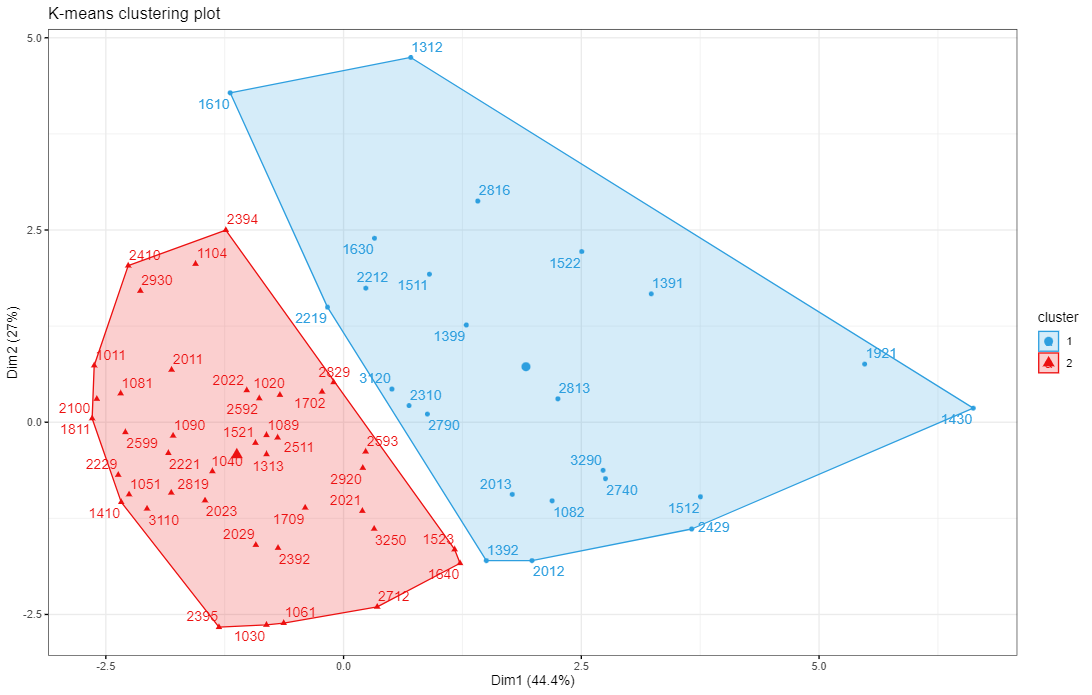
\includegraphics[scale = 0.29]{cluster.png}
		\end{figure}
	\end{frame} 
	\begin{frame}
	\frametitle{Results}
	\begin{itemize}
		\item Dim1 and Dim2
		\item Two groups: Cluster Group 1 (CG1) and Cluster Group 2 (CG2)
		\begin{itemize}
			\item \textcolor{blue}{CG1} --> n = 794
			\item \textcolor{red}{CG2}  --> n = 5192
		\end{itemize}
	\end{itemize}
	\end{frame}

	\begin{frame}[allowframebreaks]
	\begin{figure}
		\centering
		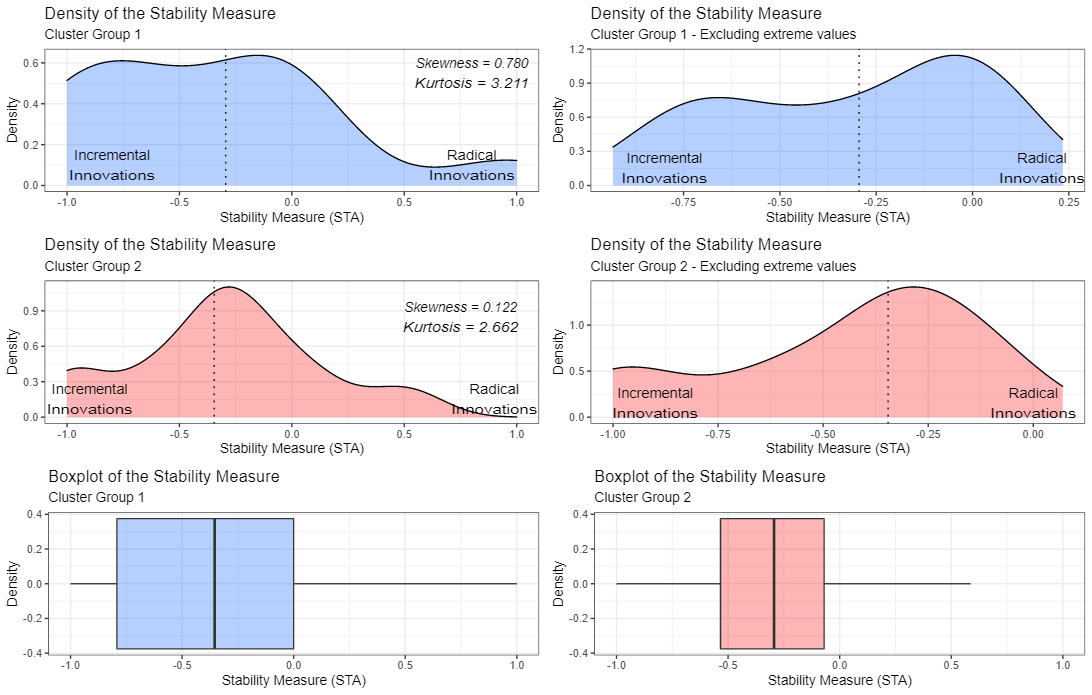
\includegraphics[scale=0.30]{sta.png}
	\end{figure}
	\framebreak
	\begin{figure}
		\centering
		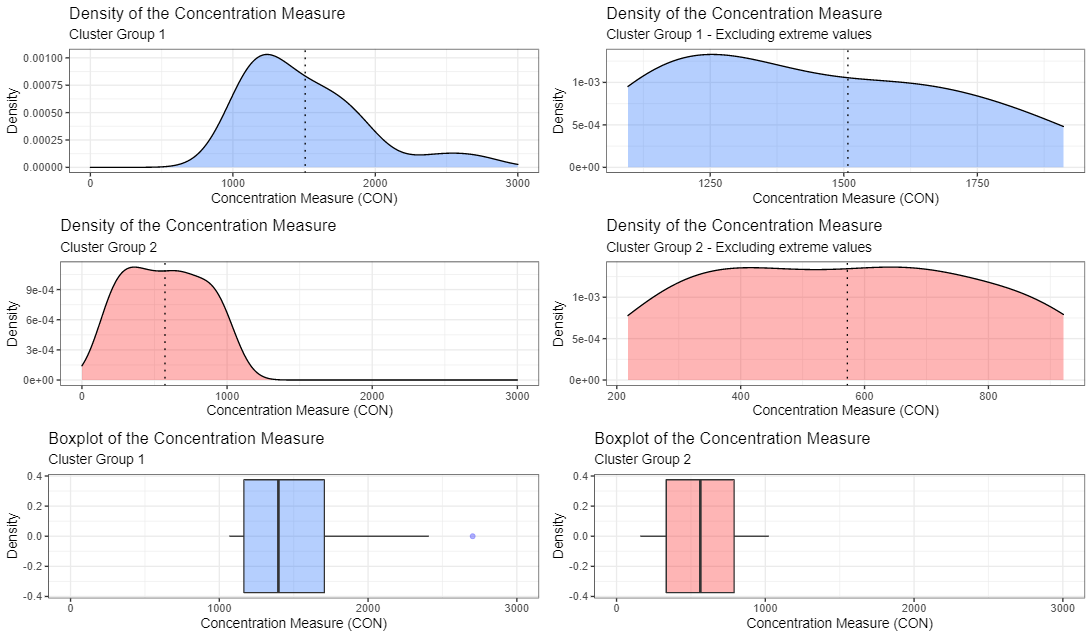
\includegraphics[scale=0.31]{pcon.png}
	\end{figure}
	\framebreak
	\begin{figure}
		\centering
		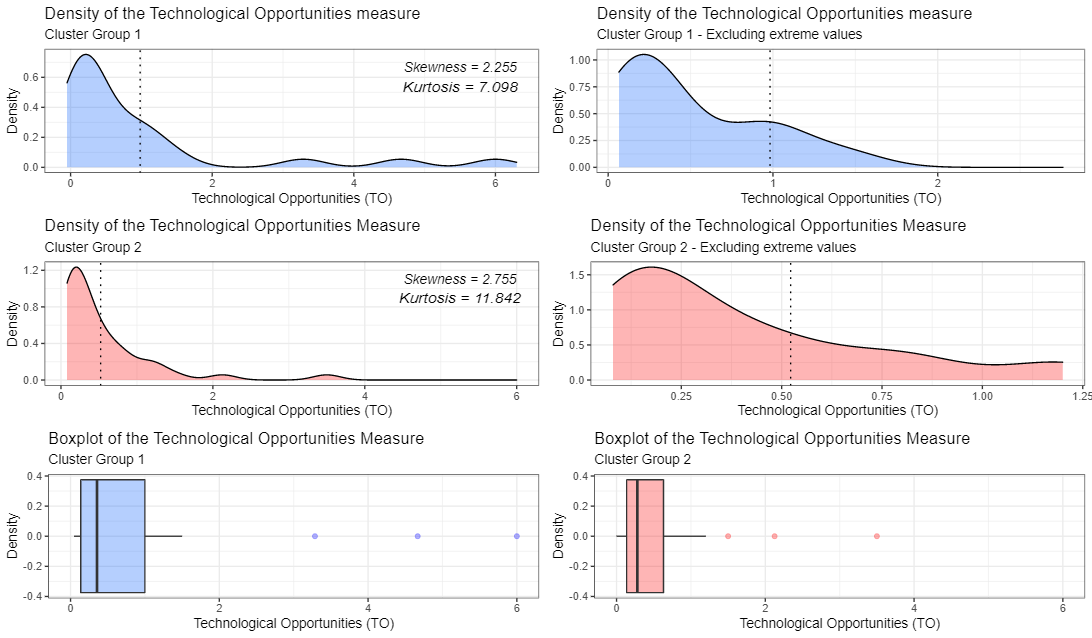
\includegraphics[scale=0.31 ]{to.png}
	\end{figure}
	\framebreak
	\end{frame}
\section{Implications}
	\begin{frame}
		\frametitle{General Implications}
		\textbf{The most important implication:}
		\begin{itemize}
			\item \textbf{\textcolor{red}{Red cluster}} (CG2): Mark I industries, small firms drive innovation
			\item \textbf{\textcolor{blue}{Blue cluster}} (CG1): Mark II industries, large firms drive innovation
		\end{itemize}
	\end{frame}
	\begin{frame}[allowframebreaks]
		\frametitle{Sectoral trends}
		Several implications for certain segments:
		\begin{itemize}
			\item \textbf{\textcolor{green}{Groceries, meat, coffee}}: Mark I. \textbf{Exception} in \textbf{\textcolor{brown}{Chocolates.}} (\textit{Nutresa?})
			\item \textbf{\textcolor{teal}{First-gen manufacture}}: Mark II. \textbf{Exception} in \textbf{\textcolor{gray}{Elaboration and finishing of clothing}}
			\item \textbf{\textcolor{olive}{Petroleum}}: Mark II (\textit{Ecopetrol?})
			\item \textbf{\textcolor{orange}{Furnitures and wood products}}: Mixed results
			\item \textbf{\textcolor{lightgray}{Metals and minerals}}: Mixed results, but more complex minerals/metals as Mark II
		\end{itemize}
	\end{frame}
	\begin{frame}[allowframebreaks]
		\frametitle{Spatial distribution}
		\begin{itemize}
			\item The article has +20 maps!
			\item \textbf{Main finding}: Centre-periphery scheme. Central Andean persists, Cauca follows. The Caribbean falls behind.
			\item \textbf{Antioquia} as the leader. \textbf{Historical factors seem to persist} (Luzardo-Luna, 2019)
			\item \textcolor{blue}{Mark II} industries are less disperse in the territory than \textcolor{red}{Mark I}
			\item \textbf{Institutionality}, \textbf{transport} access, \textbf{resource} availability and \textbf{urban} centres act as determinants of localization
			\item Yes, airports and roads are important. Magdalena navigation is also crucial, but...
			\framebreak
			\item \textbf{Institutionality seems to be the deciding factor}
			\item Where will the rule of law be enforced?
			\item Why no industries in southern Colombia? Access to \textbf{transport} and \textbf{institutionality}
			\item Why departments like Sucre, Cordoba or Cesar have little to no agglomerations? \textbf{Institutionality} and \textbf{human capital}
			\item Antioquia, prodigy kid since 1850; human capital, hard currencies, transport routes, entrepreneurship spirit. (Luzardo-Luna, 2019)
			\item So... \textbf{not one size fits all} in this matter.
		\end{itemize}
	\end{frame}
	\begin{frame}[allowframebreaks]
		\begin{figure}
			\centering
			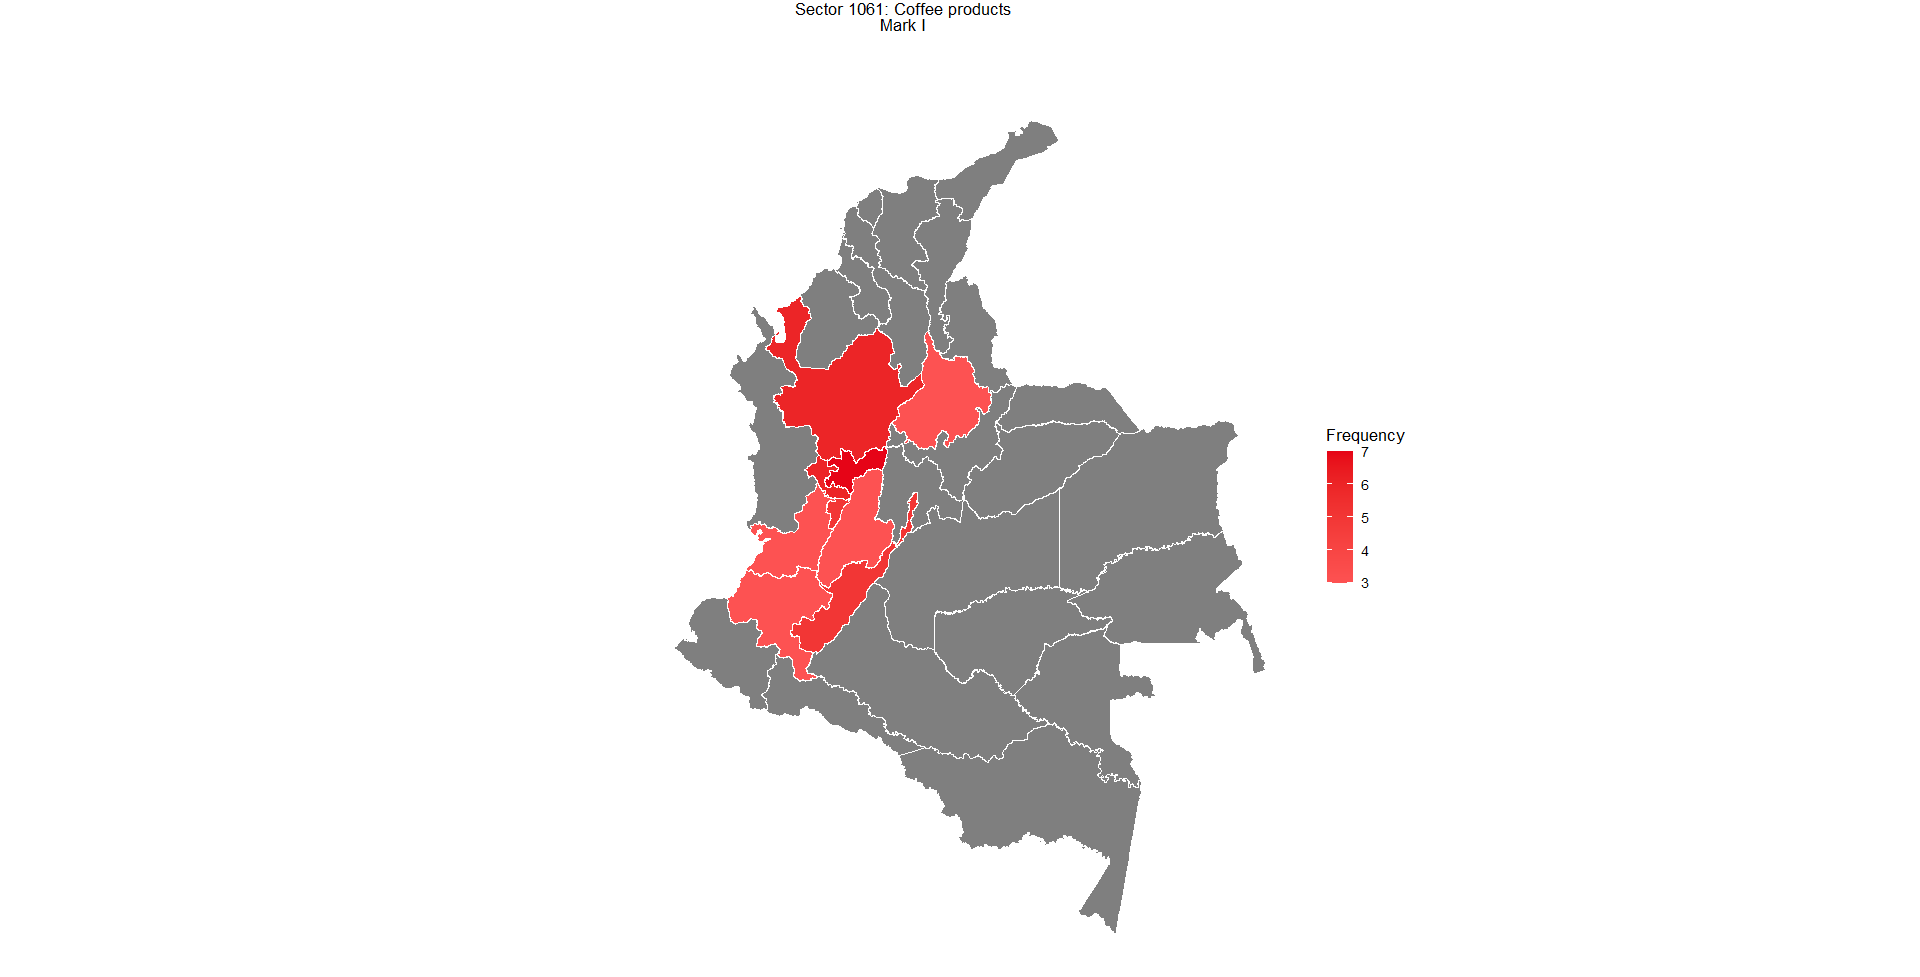
\includegraphics[scale=0.2]{coffee.png}
		\end{figure}
	\framebreak
		\begin{figure}
			\centering
			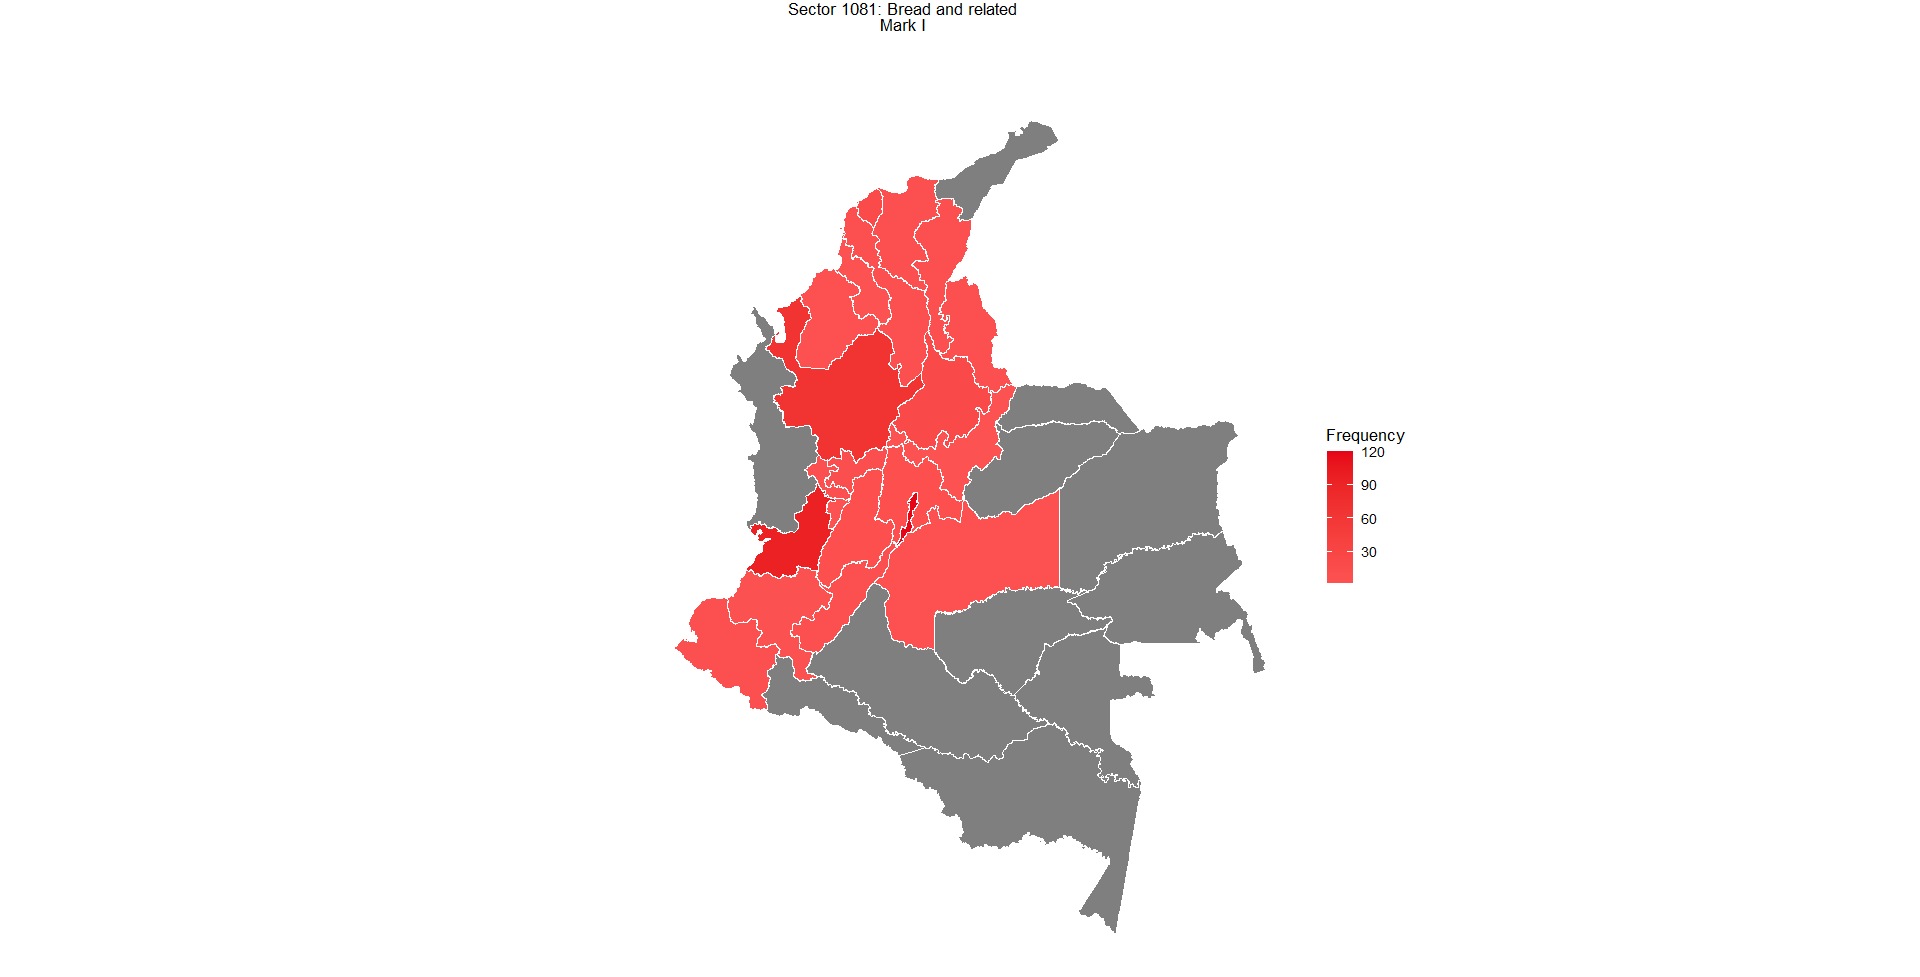
\includegraphics[scale=0.2]{bread.png}
		\end{figure}
	\framebreak
		\begin{figure}
			\centering
			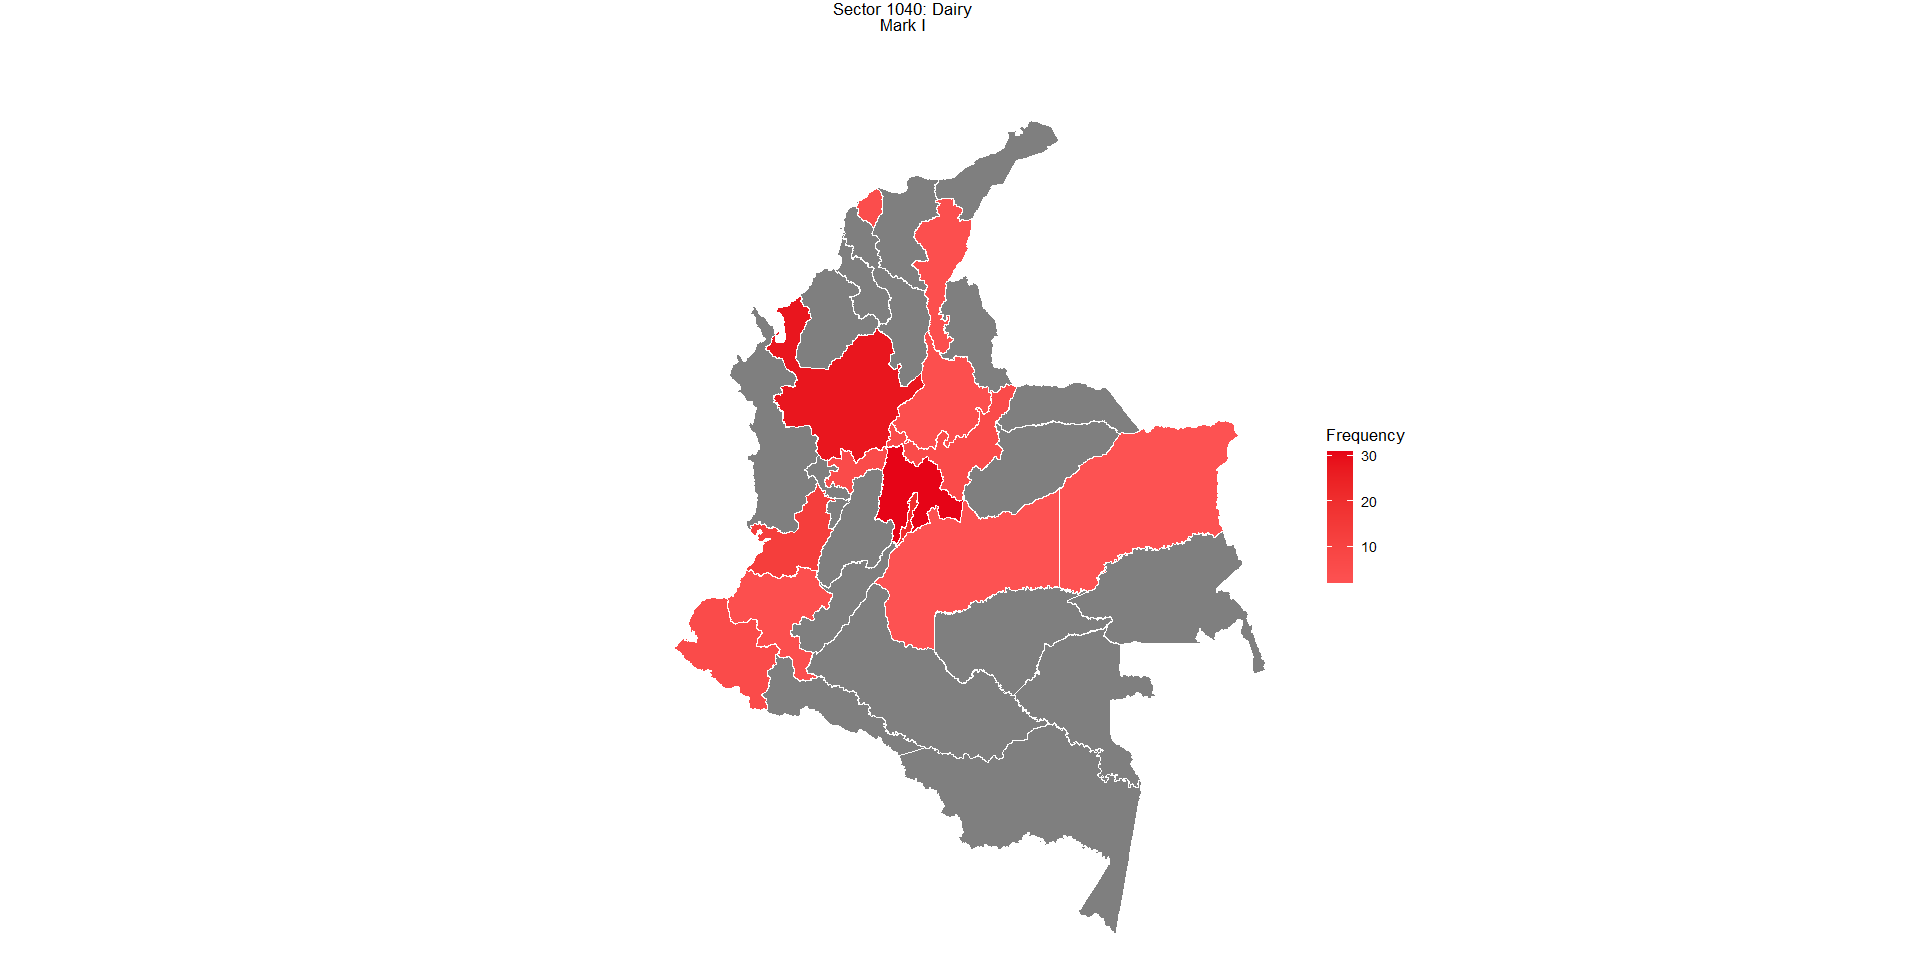
\includegraphics[scale=0.2]{milk.png}
		\end{figure}
	\framebreak
		\begin{figure}
			\centering
			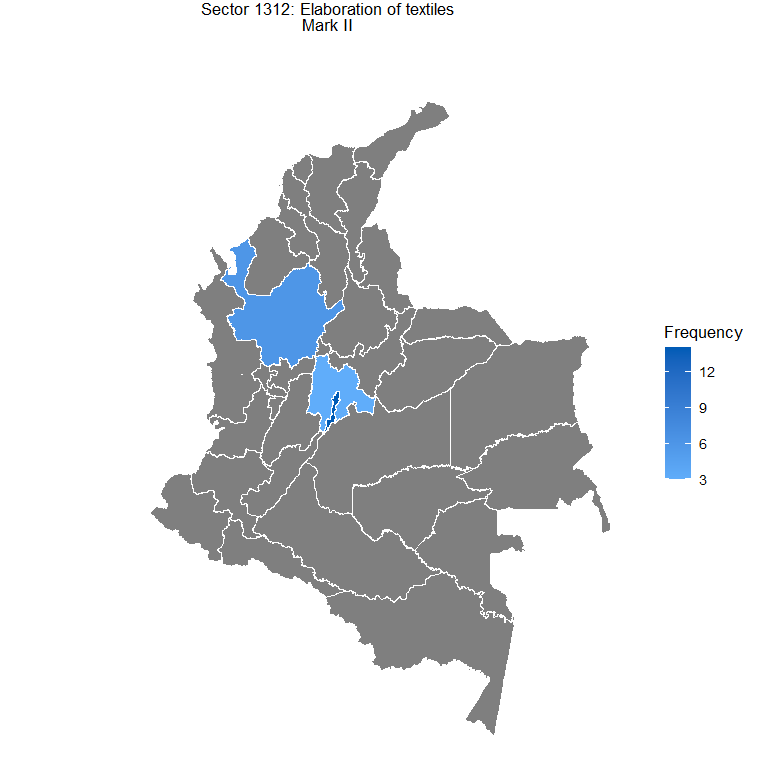
\includegraphics[scale=0.25]{textilesElabor.png}
		\end{figure}
	\framebreak
		\begin{figure}
			\centering
			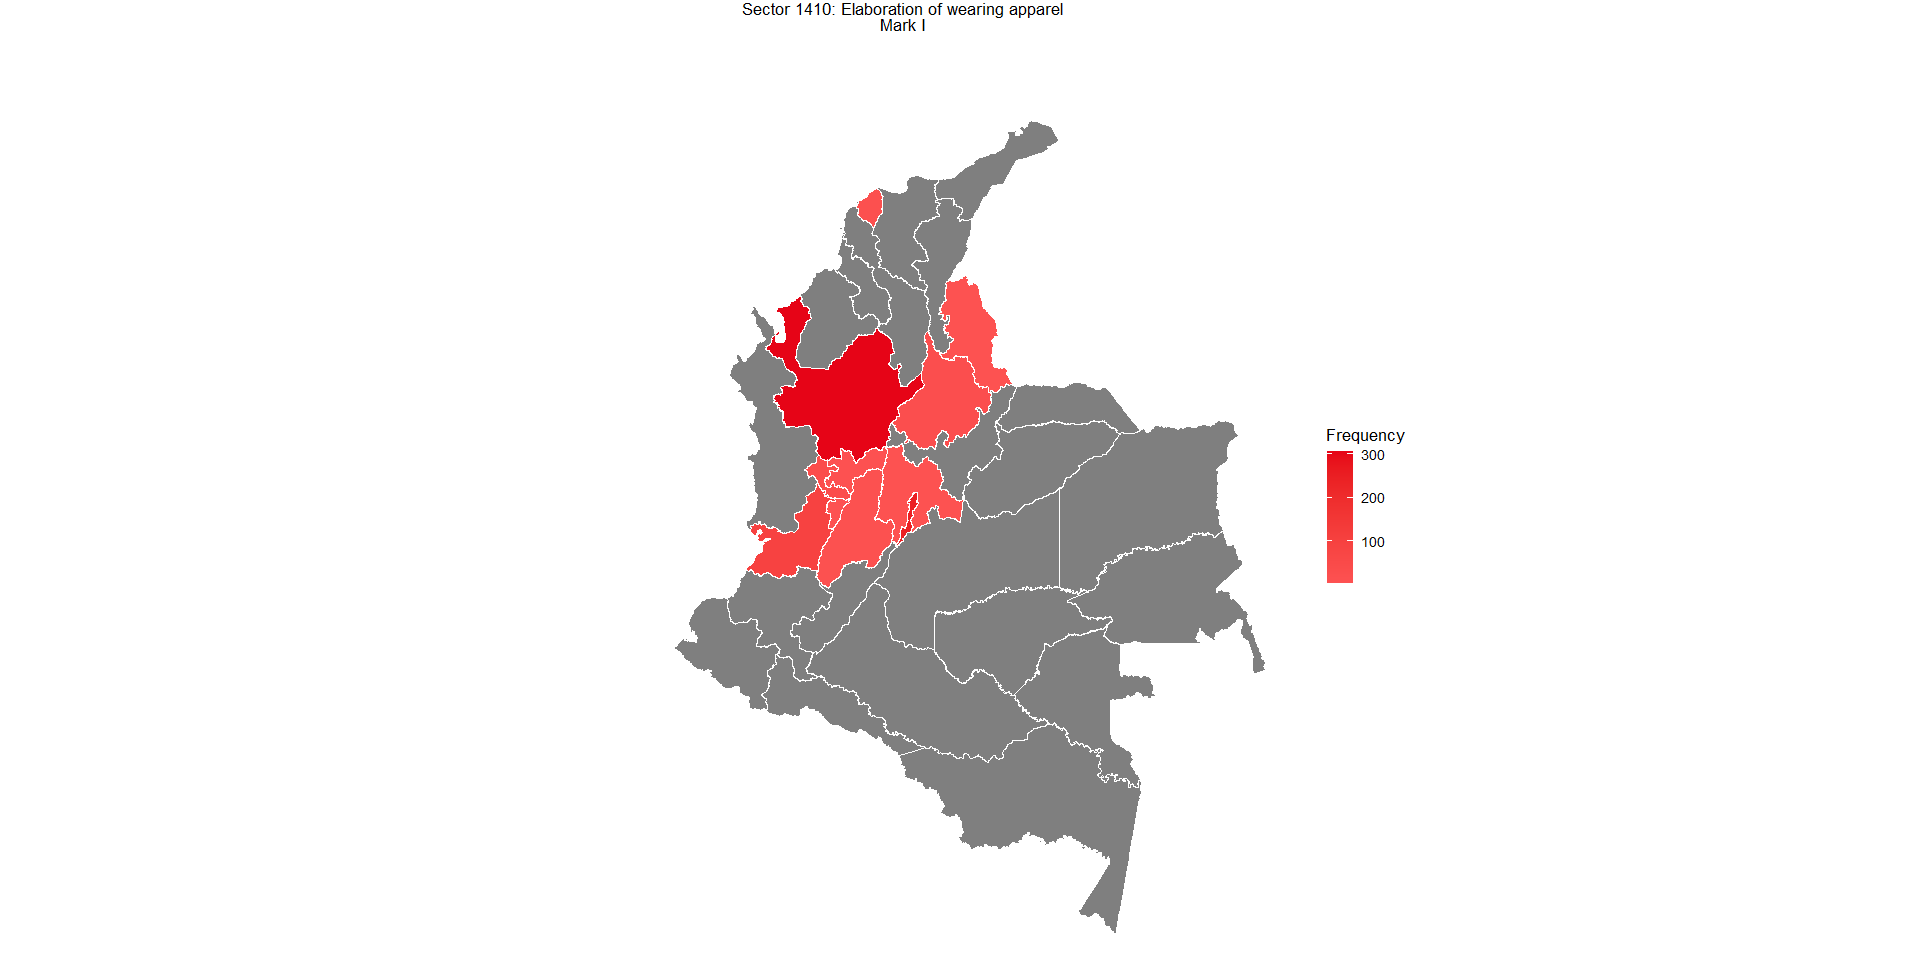
\includegraphics[scale=0.2]{wear.png}
		\end{figure}
	\framebreak		
	\begin{figure}
		\centering
		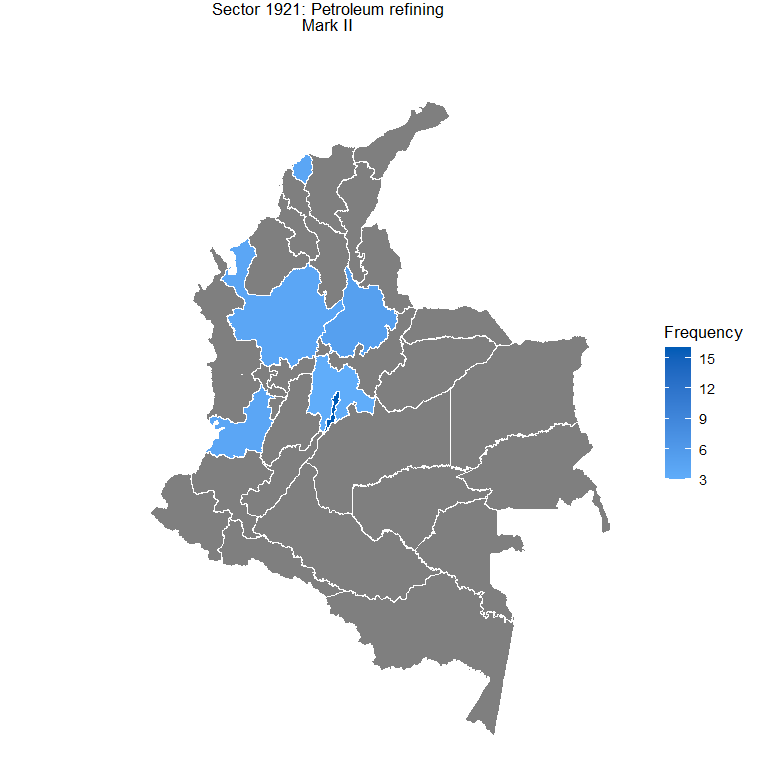
\includegraphics[scale=0.25]{oil.png}
	\end{figure}
	\framebreak
	\begin{figure}
		\centering
		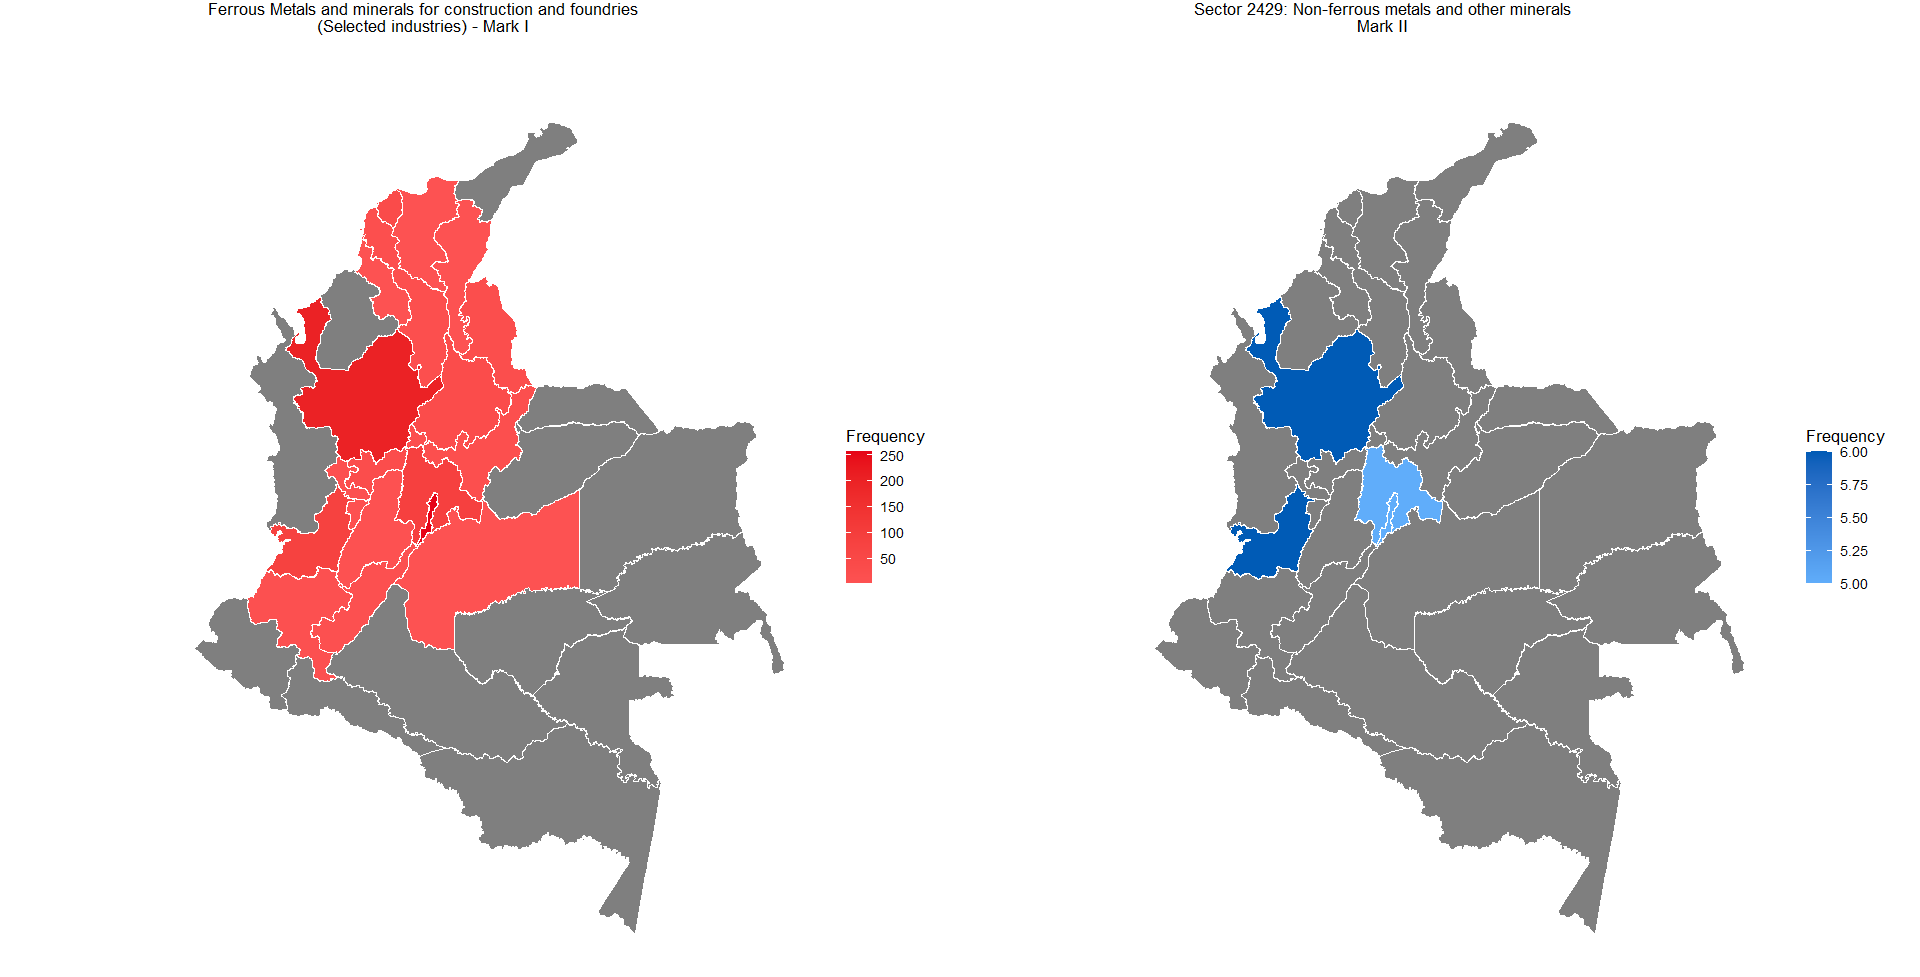
\includegraphics[scale=0.2]{metals.png}
	\end{figure}
	\end{frame}
\section{Conclusions}
	\begin{frame}[allowframebreaks]
		\frametitle{Conclusions}
		Some broad conclusions:
		\begin{itemize}
			\item We have been able to characterize Colombian industries
			\item we found what type of firm drives innovation on each industry. \textcolor{blue}{CG1} has been labeled as \textcolor{blue}{Mark II}. \textcolor{red}{CG2}, the densest group, gravitates toward \textcolor{red}{Mark I}.
			\item Measures are consistent to what was exposed in the theory and literature. Similarly, results echo with previous works.
			\item Intra-sectorial trends and geographical aspects are important for policy elaboration.
			\item Spatial distributions shows that \textcolor{red}{Mark I} industries are more disperse
			in the territory than \textcolor{blue}{Mark II} ones
		\pagebreak
			\item Policy recommendations agree on the need for heterogeneity in design, echoing with what was said about innovation systems.
			\item In other words, incentive architectures and other policy measures should acknowledge differences in geography, institutions, transport access, human capital, among others
			\item Where to channel all of this? MinCiencia's \textbf{PEDCTI} report
			\item The way forward... Econometric models, dynamic models, groundwork for policy-making
		\end{itemize}
	\end{frame}
\end{document}